\documentclass[11pt,a4paper,spanish]{book}
\usepackage{biblatex}
\usepackage[utf8]{inputenc}
% Imagenes
\usepackage{graphicx, wrapfig, hyperref}
\graphicspath{ {./.images/} }
\usepackage{float}
\usepackage{comment}
\addbibresource{./bibLib/mycol_arte.bib}
\setcounter{secnumdepth}{3}

\begin{document}
	\chapter{Desarrollo de la comparativa}
		\section{Prueba E1}
		\subsection{Conjunto de datos}
		En un primer momento los datos se han dividido por género como se especifica en el capítulo 4
		\subsection{Extracción de características}
		\begin{figure}[H]
			\centering
			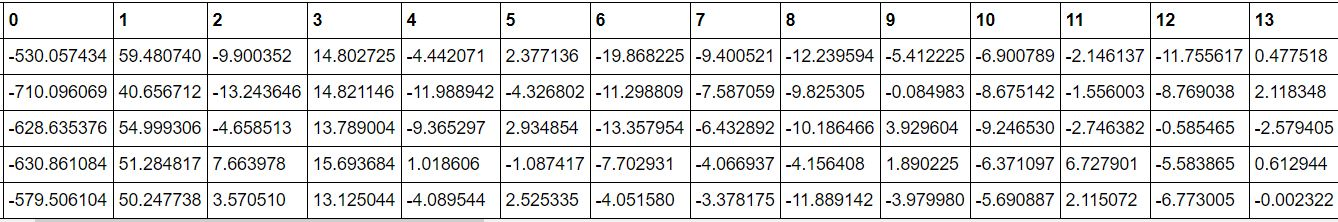
\includegraphics[scale=0.35]{featuresMFCC.JPG}
			\caption{Características MFCC extraídas del conjunto de datos}
			\label{fig:caract_MFCC}
		\end{figure}
		\subsection{Técnicas de aumento de datos}
		
		\subsubsection{Arquitectura}
		
		
		\subsection{Evaluación}
			Tras varias pruebas el modelo se simplificó considerablemente, ya que presentaba un alto sobreajuste o \emph{overfitting}. En la tabla \ref{tab:augmentationData_1} se presentan los resultados aplicados al conjunto RAVDESS con género femenino:
			
			\begin{table}[H]
			\centering
			\begin{center}
				\begin{tabular}{| c | c | c | c | c | c |}
					\hline
					Ruido Blanco & Desplazamiento & Modulación \\ 
					\hline
					 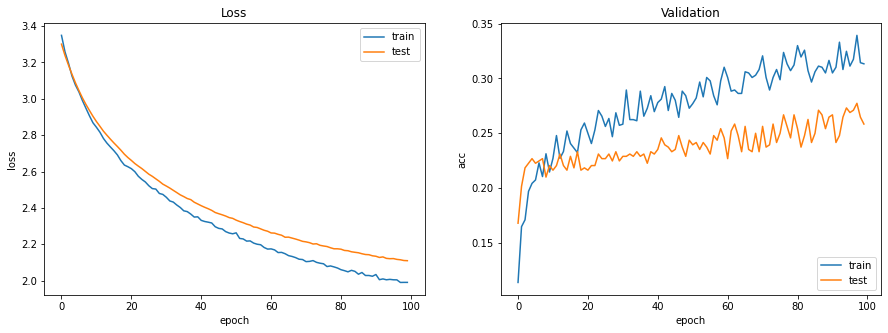
\includegraphics[scale=0.15]{results/white_noise1.png} & 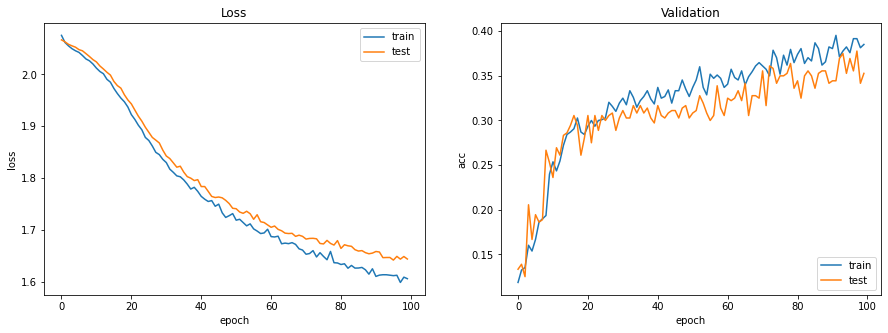
\includegraphics[scale=0.15]{results/shiftting_1.png} & 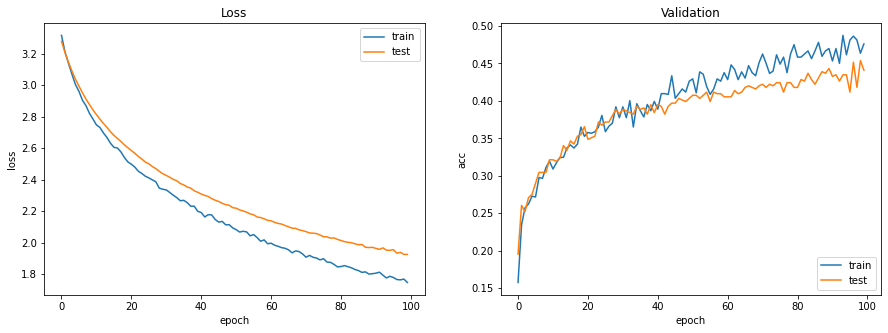
\includegraphics[scale=0.15]{results/pitch.png}\\
					
					%& & & &
					\hline	
				\end{tabular}
				\caption{Resultados obtenidos tras aplicar cada uno de los métodos de aumento de datos}
				\label{tab:augmentationData_1}
			\end{center}
		\end{table}
	
		A pesar de que dividir los datos por género parecía una buena idea, se ha comprobado que la variación en el tono provocado por el género no afecta de manera negativa al rendimiento del modelo.
		
		\begin{table}[H]
			\centering
			\begin{center}
				\begin{tabular}{| c | c | c | c | c | c |}
					\hline
					Ruido Blanco & Desplazamiento & Modulación \\ 
					\hline
					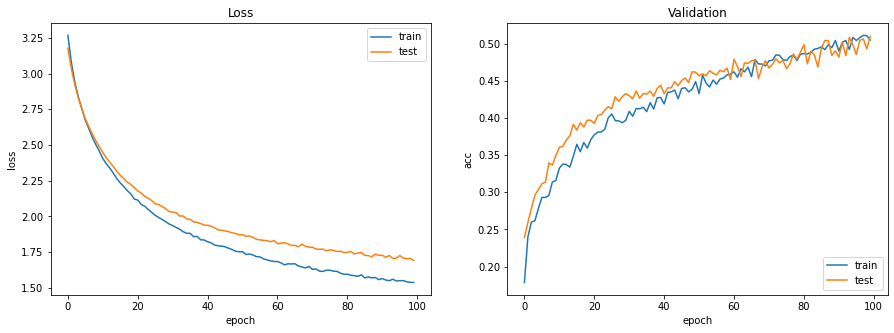
\includegraphics[scale=0.15]{results/white_noise2.png} & 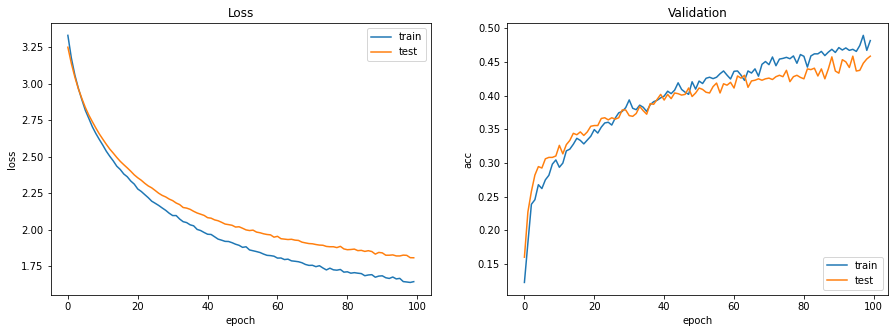
\includegraphics[scale=0.15]{results/shiftting_2.png} & 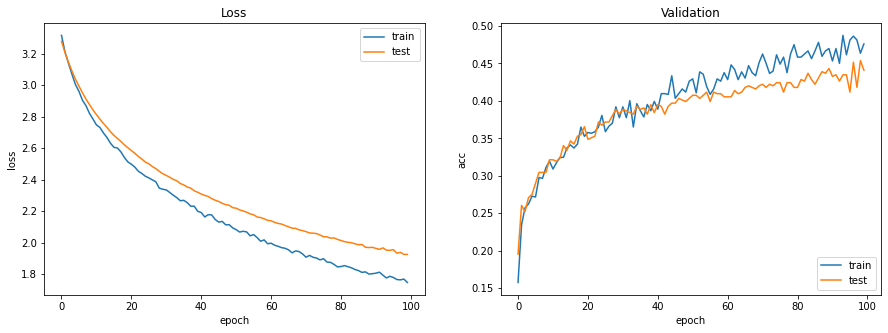
\includegraphics[scale=0.15]{results/pitch_2.png}\\
					
					%& & & &
					\hline	
				\end{tabular}
				\caption{Resultados obtenidos tras aplicar cada uno de los métodos de aumento de datos}
				\label{tab:augmentationData_2}
			\end{center}
		\end{table}
	\printbibliography
	
\end{document}